%%%%%%%%%%%%%%%%%%%%%%%%%%%%%%%%%%%%%%%%%%%%%%%%%%%%%%%%%%%%%%%%%%% 
%                                                                 %
%                      THESIS MAIN FILE                           %
%                                                                 %
%%%%%%%%%%%%%%%%%%%%%%%%%%%%%%%%%%%%%%%%%%%%%%%%%%%%%%%%%%%%%%%%%%% 

% document definition 
\documentclass[a4paper,11pt,chap,oneside]{thesis}

% Use the first command below if you want captions over 1 line indented. A side
% effect of this is to remove the use of bold for captions. To restore bold,
% also include the second line below.

\usepackage[hang]{caption2}     

\usepackage{enumitem}
\usepackage[table]{xcolor} 
%\usepackage{graphicx}
\usepackage{color} 
\usepackage{placeins}
\usepackage{transparent} 
\usepackage{hyperref}
% to indent subsequent lines of captions
\renewcommand{\captionfont}{\bfseries} 
																			 % bold caption (needed with caption 
                                       % package; otherwise bold is default)
                                       
%\includeonly{dualdynamics}  % use \includeonly to process only
                         % the file(s) listed inside the braces
                         %\includeonly{concept}
                         
% create the following file in the input from the template
\newcommand{\PaperTitle} {Probabilistic Learning of Object Locations based on spatio-temporal information }
\newcommand{\PaperSubject} {Predictive model of object locations in environment}
\newcommand{\PaperTerm} {Summerterm 2016}		
\newcommand{\PaperDate} {\today}			
\newcommand{\ThesisAdvisor} {Tim Niemueller }			
\newcommand{\ThesisReferee} {Prof. Dr. Paul Pl\"{o}ger}
\newcommand{\ThesisExReferee} {Prof. Dr. Gerhard Lakemeyer }
\newcommand{\PaperLecturerEMail} {mailto:advisor@xyz}
\newcommand{\Paperkeywords} {key1, key2, key3}		
\newcommand{\PaperMainWriter} {Deebul Nair}
\newcommand{\PaperMainWriterEMail} {mailto:deebul.nair@smail.inf.fh-bonn-rhein-sieg.de}
\newcommand{\ThesisAuthor} {Deebul Nair}

%\usepackage[latin1]{inputenc} 

\usepackage{enumitem}
\usepackage[table]{xcolor} 
%\usepackage{graphicx}
\usepackage{color} 
\usepackage{placeins}
\usepackage{transparent} 
\usepackage{hyperref}
\usepackage{tabto}


\usepackage[final]{graphicx}
%\usepackage{epstopdf}
\usepackage{url}
%\usepackage[expert,vargreek]{lucidbrb}

%\usepackage{mya4page} % not used, because now is implemented in the class 
\usepackage{amsmath}
%\usepackage{hyperref}
\usepackage{bibnames}
\usepackage{path}
%\usepackage{subfigure}

\usepackage{caption}
\usepackage{subcaption}


\usepackage{amsmath}
\usepackage{todonotes}

\usepackage{tikz}
\usepackage{amsmath}
\usetikzlibrary{bayesnet}
\usepackage{tabularx}
\usepackage{placeins}
\usepackage{pstricks}
\usepackage[titletoc]{appendix}
\usepackage{setspace}


\usepackage[nottoc]{tocbibind}
%\usepackage{footmisc}
%\usepackage[perpage,symbol*]{footmisc} 


%---------------------------------------------------------------
\usepackage{color}
\definecolor{listinggray}{gray}{0.9}
%---------------------------------------------------------------
%\usepackage[copy=false, edit=false]{pdfcrypt}

%---------------------------------------------------------------
\usepackage{listings}
\lstset{language=Java}
\lstset{basicstyle=\footnotesize\small,%ttfamily,%\small,
tabsize=4,
tab=$\to$,
float=tbph,
extendedchars=true,
breaklines,
% prebreak={\space\MyHookSign},
% frame=single,
showtabs=false,
showspaces=false,
showstringspaces=false,
keywordstyle=\color{red}\bfseries,
identifierstyle=\bf\ttfamily,
aboveskip=\bigskipamount,
}
\lstset{captionpos=b}
\lstset{keywordstyle=\color{blue}\bfseries\bf}
\lstset{backgroundcolor=\color{listinggray}, rulecolor=\color{blue}}
\lstset{linewidth=\textwidth}
\lstset{stepnumber=5}
\lstset{numbers=left}
\lstset{numberstyle=\tiny\color{blue}}
\lstset{commentstyle=\color{magenta}\textit, stringstyle=\upshape,
	showstringspaces=false}
\lstset{frame=trBL,frameround=tttt}
%---------------------------------------------------------------

%% Hyperref setup
\usepackage{hyperref}
\hypersetup{
	 a4paper,
   colorlinks=true,
   linkcolor=black,
   filecolor=black,
   citecolor=black,
   urlcolor=black,
   plainpages=false,
   pdftitle={ \PaperTitle },
   pdfsubject={ \PaperSubject },
   pdfauthor={ \ThesisAuthor <deebul.nair@smail.inf.h-brs.de>},
   pdfkeywords={ \Paperkeywords },
   bookmarksnumbered=true,
   pdfpagemode=UseOutlines,
   pdfpagelayout=SinglePage,  
   bookmarksopen=true
}
%\usepackage[copy=true, edit=false, annotate=true]{pdfcrypt}

\usepackage{fancyhdr}
\setlength{\headheight}{15pt}

\pagestyle{fancy}
\renewcommand{\chaptermark}[1]{ \markboth{#1}{} }
\renewcommand{\sectionmark}[1]{ \markright{#1} }

\fancyhf{}
\fancyhead[LE,RO]{\thepage}
\fancyhead[RE]{\textit{ \nouppercase{\leftmark}} }
\fancyhead[LO]{\textit{ \nouppercase{\rightmark}} }

\fancypagestyle{plain}{ %
  \fancyhf{} % remove everything
  \renewcommand{\headrulewidth}{0pt} % remove lines as well
  \renewcommand{\footrulewidth}{0pt}
}
%\newcommand{\picHere}[3] { %
\begin{figure}[htp] %
\begin{center} %
\resizebox{!}{!}{\includegraphics{pictures/#1}} %
\caption{{\small#2}} %
\label{#3} %
\end{center} %
\end{figure} %
}

\newcommand{\picHereWidth}[4] { %
\begin{figure}[htp] %
\begin{center} %
\resizebox{!}{!}{\includegraphics[#4]{pictures/#1}} %
\caption{{\small#2}} %
\label{#3} %
\end{center} %
\end{figure} %
}

\newcommand{\picHereRes}[3] { %
\begin{figure}[htp] %
\begin{center} %
\resizebox{!}{!}{\includegraphics[totalheight=0.8\textheight]{pictures/#1}} %
\caption{#2} %
\label{#3} %
\end{center} % 
\end{figure} %
}
 \\ not used anymore - the picture command coded directly in source

\begin{document}

%%%%%%%%%%%%%%%%%%%%%%%%%%%%%%%%%%%%%%%%%%%%%%%%%%%%%%%%%%%%%%%%%%% 
%                                                                 %
%                            TITLE PAGE                           %
%               Master's Thesis or Master's Project               %
%                                                                 %
%%%%%%%%%%%%%%%%%%%%%%%%%%%%%%%%%%%%%%%%%%%%%%%%%%%%%%%%%%%%%%%%%%% 

% Supply information for use on title page:    
\thesistitle{\bf Predicting Object Locations using Spatio-Temporal Information by a Domestic Service Robot: A Model Based Machine Learning Approach }
%used for the header
\thetitle{Predictive model of object locations in environment}         
\author{\ThesisAuthor}        
\degree{Master of Science in Autonomous System}
\thadviser{\ThesisAdvisor}
\cothadviser{\ThesisReferee}
\exthadviser{\ThesisExReferee}
\submitdate{March 2016}
\copyrightyear{2016}   % if omitted, current year is used.        

% Print titlepage and other prefatory material:   
\titlepage        
%\copyrightpages
%\emptypage         %optional 
%\statementpage         
%\emptypage
% toc, abstract, acknowledgement 
\singlespace 
%%%%%%%%%%%%%%%%%%%%%%%%%%%%%%%%%%%%%%%%%%%%%%%%%%%%%%%%%%%%%%%%%%% 
%                                                                 %
%                            ABSTRACT                             %
%                                                                 %
%%%%%%%%%%%%%%%%%%%%%%%%%%%%%%%%%%%%%%%%%%%%%%%%%%%%%%%%%%%%%%%%%%% 
\begin{abstract}


In the future, we envison domestic robots to provide useful services both in domestic as well as in industrial context. Examples include domestic service robots, that implements large part of our housework, versatile assistants, that provide automation, transportationm inspection and monitoring services. The challenge in these aplications is that the robots has to have lot of information and knowledge about the user and environment to operate under complete autonomy.This thesis aim is to enable domestic robots to acquire knowledge about behaviour and preferences of the users around them. The developed approaches in this thesis cover the following two topics: (1) learning about the temporal human location behvaiour in-door using previously observed locations of the human (2) learning user preference in object placement. 
 
All techniquies developed in this thesis are based on probabilistic bayesian learning and inference. They have been implemented and evaluated on datasets  collected using real robots as well as on simulated datasets. Extensive experiments have been conducted to evaluate the and validate the properties of the proposed models.
\todo{need to be revised completely}
\end{abstract}
\onehalfspace
%\emptypage
%%%%%%%%%%%%%%%%%%%%%%%%%%%%%%%%%%%%%%%%%%%%%%%%%%%%%%%%%%%%%%%%%%%% 
%                                                                 %
%                         ACKNOWLEDGEMENT                         %
%                                                                 %
%%%%%%%%%%%%%%%%%%%%%%%%%%%%%%%%%%%%%%%%%%%%%%%%%%%%%%%%%%%%%%%%%%% 
 
\specialhead{ACKNOWLEDGMENTS}
 
ACK. ACK. ACK. here you can write your acknowledgements. 

%\emptypage

\tableofcontents 
\pagestyle{plain}       
\newpage
\emptypage
%\listoftables          %required if there are tables
%\listoffigures         %required if there are figures
   

% the main contents %
\chapter{Introduction}


For robots to make a smooth ingress into dynamic human environments like home and office, the robots need to be able to close the \emph{perceive-action-learning} loop. Essentially these domestic service robots should perceive the environment, interact with the environment, learn from experiences and repeat. The robot interacts with the environment by choosing a sequence of low-level actions . For example, lets take the high-level task of ``making tea", this will require the following actions to be executed sequentially: fill the kettle, boil water, find the teabag, find a cup, put teabag into the cup and pour hot water into the cup. But for executing some of the actions like finding the kettle, finding teabag, finding cup etc. requires the robot to have prior knowledge about the possible locations. Such knowledge about the environment or the user needs to be learned by the robot. The goal of this thesis is to enable domestic service robots to gain knowledge about common behaviours and preferences of the user in a non-intrusive manner. Specifically, we address how Bayesian methods can be used to provide a flexible and computationally efficient structure for acquiring knowledge using limited spatio-temporal information collected by these service robots.

Domestic service robots need to have the ability to automatically and quickly adapt to a new environment. Imagine if the robot could learn how the user arranges the breakfast table by looking at the data from previous days? Robots can observe our lives and provide small insights the user doesn’t even notice. The robots can pass along helpful information to the users, like observing their sleep habits and tell us when we are not having adequate sleeps. By learning how the user interacts with their homes and how they live their lives, robots will be able to provide better services to their users. 


Domestic service robots while interacting with the user and environment produce information which after being processed in perception, actuation, or decision making are discarded. \cite{niemueller2012generic} has proposed an approach of storing these information in a robot database and produce useful knowledge. 
The domestic robot will continuously record sightings of objects and persons with position and time in a database to form the spatio-temporal robot memory. Machine learning is a good method for automatic knowledge generation from the stored information. But in order to adapt quickly the robot needs to able to extract valuable knowledge from small amount of information, i.e., the learning algorithms need to be data efficient.

To illustrate the relevance of the topics presented in this thesis, we motivate our work using a typical task of a domestic service robot.   We assume that the robot is given the task of ``making coffee" for the user Waldo, which requires the robot to locate the coffee cup of Waldo first, make coffee and then to locate Waldo for delivering it to him. To begin the search for the coffee cup, it would help the robot to have some prior knowledge regarding Waldo's habits; in particular the typical locations where he keeps his cup. This enables the robot to funnel its search for the object from a large number of locations to the most probable ones. Once the coffee cup is located and grasped the robot needs to reason about where it can currently find Waldo for delivering it to him. This in turn, requires the robot to have knowledge about the likely locations of Waldo at that time.

This motivating example leads us to the two research topics in knowledge acquisition we address in this thesis:
\begin{enumerate}
	\item How can a domestic service robot acquire knowledge about user preferences in placing objects in the environment?
	\item How can a domestic service robot acquire knowledge about the user's temporal location behaviour?
	\item How can a domestic service robot acquire the above knowledge using small amounts of information?
\end{enumerate}

A service robot operating in dynamic human environments needs to perceive the world using its own sensors, and subsequently build a cognitive model of the user preferences and behaviour. These models represent the internal beliefs of the robot about the user preferences and behaviour. The model needs to be extract the knowledge from small amount of information, basically we should develop methods to do data-efficient machine learning. There are many approaches that demonstrate that data-efficient machine learning is possible, including methods that: explicit domain knowledge, exploit structural knowledge of data, bootstrapping and data augmentation, semi-supervised learning, transfer learning, active learning and Bayesian optimization, non-parametric methods, one-shot learning and Bayesian deep learning \cite{https://sites.google.com/site/dataefficientml/home}. 
Bayesian probabilistic formulation of the cognitive model makes it possible to include the above mentioned methods in a single framework. The robots can use these models to predict the future behaviour of the user or can make educated guess about the user while doing actions with partial information.


In sum, this thesis provides Bayesian probabilistic techniques that enable a domestic service robot
\begin{itemize}
	\item to learn the user preference model in object placement.
	\item to learn the user's temporal location behaviour model.
	\item to learn in the absence of information.
\end{itemize}

\todo[inline]{should we add chapter flow?}

All of our approaches are based on state-of-the art Bayesian learning techniques such as Dirichlet processes, graphical models and probabilistic programming. The probabilistic formulation of our approaches allows the robot to represent the state of its knowledge or the state of its belief. In an exhaustive set of experiments on real-world and simulated datasets we show that our approaches are able to successfully extract knowledge about user behaviours and preferences from observations made by a domestic service robot. Furthermore, we also demonstrate that the acquired knowledge can be utilized in smart decision making frameworks to reduced the time required to complete each tasks. We hope that our approaches will set up service robots into the existing household by knowing what and who is there and adapting to them. Service robots will grow and change with the users, with a greater awareness of the world around them



%%%%%%%%%%%%%%%%%%%%%%%%%%%%%%%%%%%%%%%%%%%%%%%%%%%%%%%%%%%%%%%%%%%%%%%%%%%%%%%%%%%%%%%%%%%%%
% 																STATE OF THE ART 																					%
%%%%%%%%%%%%%%%%%%%%%%%%%%%%%%%%%%%%%%%%%%%%%%%%%%%%%%%%%%%%%%%%%%%%%%%%%%%%%%%%%%%%%%%%%%%%%
\chapter{STATE OF THE ART}

The problem of modelling object location in the environment is mostly studied as a subtopic to other topics like Active Object Search, Active Visual Object Search, Exploration technique, World Model and World State Estimation.

\begin{figure}[htp]
\centering
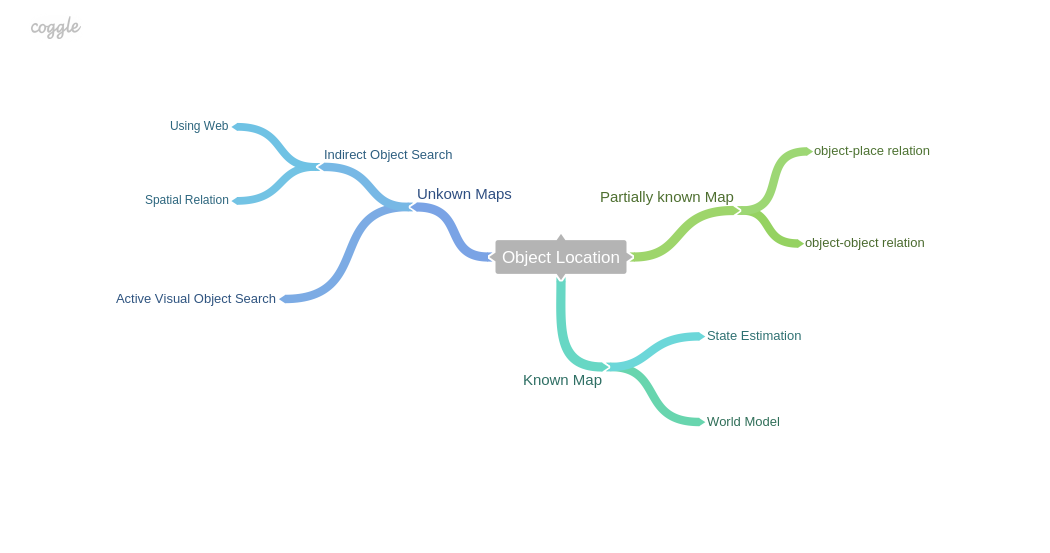
\includegraphics[scale=0.45]{pictures/Object_Location.png}
\caption{Related Work Overview}
\label{Related Work}
\end{figure}

Robots in a human-centric indoor environment need continuous interaction with the environment. The robots need to have relevant information about the objects in the environment. As a result major chunk of the research in robotics has been in this problem of searching for objects in the environment.
We start with a comprehensive treatment of the early and current work related to the object location modelling scenario that is considered in this work. This allows us to show how our work fits into this and how it pushes the state of the art.

For the purpose of clarity the literature is divided into the following categories mainly : 
\begin{itemize}
	\item Object location of novel objects 
	\item Object location of partially known objects
	\item Object location of already known non-stationary objects
\end{itemize}
\subsection{Novel objects}
\label{sub:novel objects}
In all these works the robot has no previous knowledge about the environment and instead relied on prior information of generic indoor spaces or heuristics based exploration strategy to search for novel objects. 
In the seminal paper, Bajcsy introduced the term active perception \cite {bajcsy1988active}. The focus was to move from just perceiving to searching while perceiving.

\cite{wixson1994using} recognized that searching indirectly for 'intermediate' objects can make search more efficient and provided qualitative results by comparing two search strategies. This work inspired many such other search strategies and were called as "Indirect Object Search". 

In a series of papers \cite{aydemir_plan-based_2011} \cite{aydemir_exploiting_2012}and others in the CogX project 
extended the indirect object search by introducing spatial relations to define object targets relative to landmarks.

\cite{kunze_indirect_2014} extended this approach by using probabilistic models of qualitative spatial relations to improve the object search task.
The most recent work in \textbf{Active Visual Search Problem(AVS)} is by \cite{aydemir_active_2013}, in which they have provided an comprehensive overview of the field. This work combines semantic information about the object and environment to derive better search strategy. They have compared their approach to all the existing AVS search strategies.
% subsection novel objects (end)

\subsection{Partially known objects}
\label{sub:partially known objects}
Object contextual information for searching objects as been repeatedly proven good results. Many search strategies involving searching based on known object locations have been developed
\cite{kollar_utilizing_2009} utilize object-object and object-place co-occurrences probabilities as a way to shape the prior on the object location over the search space. Using prior map of the environment and knowledge about some of the objects in it, they try to search for location of novel objects.
Extension to this approach involving information retrieval from the web has been explored by \cite {samadi_using_2012}
\cite{kunze_searching_2012} applied the semantic similarity measure for object search by using prior information from a web-trained ontology.
Finally, \cite{joho_learning_2011} illustrated one way of combining both types of information by extracting features to train a reactive search heuristics.

\cite{wong_using_2014} considered the case of occluded objects. Occluding objects in the front typically need to be moved away to enable further perception and eventual discovery of such occluded objects. 
% subsection partially known objects (end)

\subsection{Known Non-stationary Objects}
\label{sub:known non-stationary objects}
For successful execution of task for mobile-manipulation robots, should have a estimate of the state of the environment. \cite{elfring_semantic_2013} have addressed this problem by creating a model based object tracking framework. It tracks objects in the environment by modelling the uncertainty in the object location.
\cite{wong_manipulation-based_2013} have proposed a world model representation based on the objects. 
\cite{krajnik_wheres_2015}  propose a novel  approach  to  mobile  robot
search  for  non-stationary  objects  in known  environments. They use spatio temporal models for object locations .
This approach, forms the baseline for comparison of our models. Its the only approach in which long-term data from a single environment is used to make analysis of the object locations. They argue that the  probability of object occurrences at particular locations is function of time.


% subsection known non-stationary objects (end)

\subsection{User Preferences}
\label{sub:user preference}
Researchers have tried to figure out the challenges which will be involved in
placing robots in a human environment.\cite{pantofaru_exploring_2012} conducts
interviews with people to understand the needs of people with robots. One of the
suggestion was help in organizing things based on the user preferences.
For understanding user preferences in organizing objects in home work has 
been done by  \cite{abdo_collaborative_2014}, where robots learn about user
preferences in organizing objects. The learning uses data collected by 
crowdsourced data collected from thousands of users to predict location of 
novel objects. Our work differs from above as we only use data collected from a single home and predict object locations for the same home. Thus the learning is to understand and reason about a single home and not about a generalized home.

% subsection user preference (end)

% section Related Work (end)

\section{Contribution}
\label{sec:contri}
Most of the related work till now has concentrated on predicting object location for a generalized home. The data is collected for different homes together and then learning is applied generally for all homes collectively.  This work will contribute towards learning object locations for a specific home. It will do data collection in a single home and create predictions for the same. The model will thus capture the user preferences in the usage of space.

The approach proposes a way of integrating data of object location captured at
different times and locations into a dynamic spatio-temporal model and uses the
model to predict the future location of the objects. The proposed model will be
able to learn, predict, observe, relearn and refine the object locations which
enables efficient object search.


% section contri (end)
 

%%%%%%%%%%%%%%%%%%%%%%%%%%%%%%%%%%%%%%%%%%%%%%%%%%%%%%%%%%%%%%%%%%%%%%%%%%%%%%%%%%%%%%%%%%%%%
%\chapter{PROBLEM STATEMENT} -- not always required the chapter name as problem statement.	%
% chapter problem statement - in this chapter the problem of the thesis are desribed.				%
%%%%%%%%%%%%%%%%%%%%%%%%%%%%%%%%%%%%%%%%%%%%%%%%%%%%%%%%%%%%%%%%%%%%%%%%%%%%%%%%%%%%%%%%%%%%%
\chapter{OBJECT LOCATION MODEL} 

\section{Probabilistic Modelling}
\label{sec:probability modelling}

Can machines learn from experience? Machine learning as a science has been trying to find a answer to the question from its inception. Machine learning is building knowledge from the data. One approach of building knowledge from data can be to learn the process which generated the data we have observed by creating a model of the process.
\textbf{Probabilistic Modelling} gives us a framework in which we can create such a model, based on our assumptions of the process. The model is basically expressing the assumptions in a mathematical form. The assumptions are the number of variables in the model, the relation between these variables, changes in which variables affects which other variables. This model is then used to generate a problem specific algorithm which can be used to solve the machine learning problem in hand. 

\subsection*{Steps required in Probabilistic Modelling}
\label{sub:steps}
\begin{enumerate}
	\item \textbf{Gather data} to be used for training and evaluation.
    \item \textbf{Gather knowledge} required for model building.
    \item \textbf{Visualise} the data to understand it. This is useful also for gathering knowledge. After visualization the insight gained can be used for assumptions in model building.
    \item \textbf{Construct a model} based on the knowledge of the problem statement available and data visualization. 
    \item \textbf{Perform inference} using both the data and the constructed model. The variables of the model are tuned based on the data available. Predictions can be made to find out the knowledge gained by the model.
    \item \textbf{Evaluate} the performance of the model based on evaluation metric.
    \item \textbf{Diagnose} the model and the assumptions if the evaluation is below some acceptable range
    \item \textbf{Refine the system} by adapting different model structure, inference engine

\end{enumerate}
% subsection steps (end)


\begin{figure}[htp]
\centering
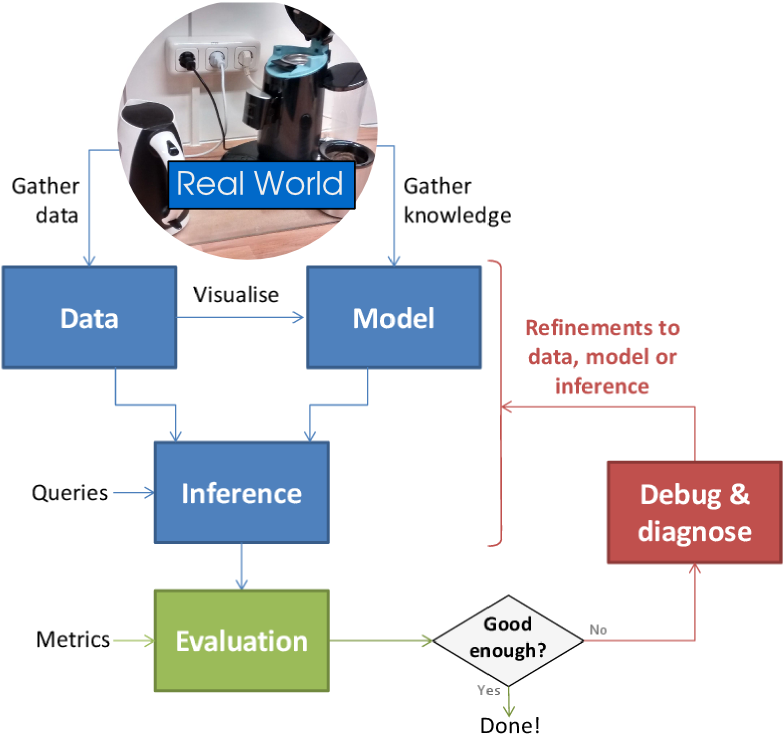
\includegraphics[scale=0.5]{pictures/Lifecycle.png}
\caption{Steps involved in probabilistic modelling  \url{ http://www.mbmlbook.com/LifeCycle.html}}
\label{}
\end{figure}




% section probability modelling (end)
\FloatBarrier
Predicting object location based on the previous seen observations has a lot of challenges. 
\begin{itemize}
	\item  Sparse dataset:-\\
Since the robot is moving around the home and recording the position of objects it has perceived the dataset on which learning has to be performed is sparse. Classical pattern recognition like PCA(eigen vectors)
and variable hidden markov model will not be able to find pattern in such
sparse dataset. We therefore need a method that can fill in (extrapolate from
observations) large periods of no observability.
    \item Occlusions :- \\
Not only the observations are sparse because of less observations, there is great
sparsity because of occlusions. In a home scenario most of the objects are
always inside containers which cannot be perceived.
    \item Over fitting :- \\
Over fitting is a danger when the number of observation available for learning
is so sparse.
\end{itemize}

As suggested classical machine learning algorithms for finding patterns will not be successful because of the sparseness in the dataset.
The considerations suggest the use of Model based machine learning framework   which allows us to overcome the sparseness in the dataset by creating models and providing some prior information available about object locations in the model.
Furthermore Bayesian non-parametric methods can provide with powerful guards
against over fitting

\section{Problem Formulation}
\label{sec:Problem formulation}

The problem can be formulated as getting an accurate predictive probability density of possible object locations given the previous object locations and the time. Given the corresponding observations of $D_{o_i}$, the probability distribution over the object locations of $o_i$ at time $T$ is governed by the following formula 

    \begin{equation} \label{eq:1}
	    P(l_i | t_i, D_{o_i})
    \end{equation}

   Various temporal information related to periodic patterns can be implied by $T$, to indicate the object's location. Such as specific hours of the day (11:00 pm), a day of the week(Friday), or a month of the year(February). We use the \textbf{temporal state} to represent such information and introduce $r(t)$ to denote temporal state extracted from time $T$,.  Dependency on the type of the temporal state $r(t)$ can be a different function. For example,if $r(t)$ denotes temporal state in terms of hours of the day then $r(t) \in {0,1 ... , 23}$, if $r(t)$ denotes temporal state in terms of day of the week, then $r(t) \in {0,1, .. 6}$ . Without loss of generality, we use $r(t)$ to denote a type of temporal state in the following description, Equation \ref{eq:1} is reformulated as 
    
    \begin{equation}
	    P( l_i | r(t), D_{o_i})
    \end{equation}
    
    Applying Bayes Rule
    
    \begin{equation}\label{eq:3}
	P( l_i | r(t), D_{o_i}) \propto P(r(t) | l_i, D_{o_i})  P(l_i | D_{o_i})
    \end{equation}
    Where:
    \begin{itemize}[label=]
    \item $P(r(t) | l_i, D_{o_i})$ : Temporal context 
    \item $P(l_i | D_{o_i})$ : Spatial context
    \end{itemize}
    
     The spatial context $P(l_i | D_{o_i})$ indicates the location distribution of object $o_i$ given the previous observed location $D_{o_i}$ . The temporal context $P(r(t) | l_i, D_{o_i})$ represents the temporal state distribution of object $o_i$, being observed at location $l_i$ with corresponding $D_{o_i}$
    


\begin{tabular}{cp{8cm}}
    \hline
	Symbol & Meaning\\
	\hline
	O & Set of all Objects\\
	$o_i$ & Single object from the set $O$, $o_i \in O$ \\
	$L$ & Set of all Locations\\
	$l_i$ & Single location from the set $L$. $l_i\in L$\\
    $T$ & Time interval\\
    \hline
	$<o_i,l_i,t_i>$ & Object $o_i$ was located at location $l_i$ at time $t_i$\\
	$D$ & Collection of all objects all observed locations\\
	$D_{o_i}$ & Previous observed locations of $o_i$\\ 
    \hline
     $P(r(t) | l_i, D_{o_i})$ &  Temporal context representing the temporal state distribution of $o_i$ at location $l_i$ given previous observations $D_i$\\
     $P(l_i | D_{o_i})$ & Spatial context representing the location distribution of object $o_i$ given the previous observations $D_{o_i}$\\
    \hline
\end{tabular}
% section Problem formulati (end)

\section{Proposed topics of study in the thesis }
\label{sec:Proposed study}
\begin{itemize}
	\item Temporal Preferences :- $P(r(t) | l_i, D_{o_i})$ \\
	Represents the effects of temporal preferences. It captures the temporal state of a object placement at a location based on the previous observations of the object so far.
	\item Spatial Preferences :- $P(l_i | D_{o_i})$ \\
	Represent the effect of spatial preferences. It captures the location preference of the user where he/she likes to place the object at location $l_i$ based on the previous observations of the object so far.
	\item Temporal-Spatial Co-relation : \\
	\ref{eq:3} combines both the user's temporal context and spatial context corresponding to the co-relations between temporal cyclical information and chronological information.
\end{itemize}
% section  Things to study (end)

\newpage
\section{Proposed Models}

This section mentions the various models which can be used to model the spatio-temporal pattern generation:

\subsection{Gaussian Mixture Model based Naive Bayes Classifier}
\label{sub:GMM}
One of the hypothesis to be examined in the thesis is that the object location has a temporal pattern. The objects locations are decided on the basis of time. For our thesis we will analyse two different type of temporal cyclic patters(daily and weekly).
Since we don't have the location of objects all the time smoothening technique is inevitable to evaluate the probability of a object location at unobserved times.
Mathematically we need a probability distribution to model a user's temporal preference at location $P(r(t) | l_i, D_{o_i})$ . Such distributions should satisfy the following requirements:
\begin{itemize}
	\item Probability distribution centres on one or more temporal state
	\item Probability decreases as the distance to the centre point increases
	\item Each object has a biased probability decreasing speed around the centre
\end{itemize}

Gaussian Mixture Model (GMM) capture these properties.

\subsubsection*{Temporal Cyclic Pattern}
\label{ssub:}
We first formally define $r(t)$ in terms of daily and weekly temporal states. We define $r(t) = {r_d(t), r_w(t)} $ as two indicator function mapping. The timestamp for each type of time where $r_d(t) \in {0,1 .. 23}$ and $r_w(t) \in {0,1 ... 6}$.

So the temporal state can be re-written as :
\begin{equation}
	P(r(t) | l_i, D_{o_i}) = P(r_d(t), r_w(t) | l_i, D_{o_i})
\end{equation}
We will follow independence assumption of daily and weekly patterns.
\begin{equation}
	P(r(t) | l_i, D_{o_i}) = P(r_d(t)| l_i, D_{o_i}) P(r_w(t) | l_i, D_{o_i})
\end{equation}

\begin{figure}[htb] 
\centering 
\def\svgwidth{200pt} 
\input{bayes-model.pdf_tex} 
\caption{Graphical structure of Temporal Cyclic Model. Shaded nodes are observed} 
\end{figure} 
% subsubsection  (end)
% subsection GMM (end)

\FloatBarrier
\subsection*{Dirichlet Process Mixture Model}
\label{sec:dp model}
In this model we assume that the latent discrete locations $l_i$ is not known to us. We would infer this directly from the observations.
Mixture modelling is a well established method for inferring latent discrete variables when we know exactly the clusters involved.
Therefore we use Dirichlet process mixture model that allows us to infer the number of locations, k.

Again, even here to address the problem of filling in large period of missing data, we assume the behaviour is periodic.
% section  (end)
\begin{figure}[htb] 
\centering 
\def\svgwidth{450pt} 
\input{lda-model.pdf_tex} 
\caption{Graphical structure of Latent Dirichlet Model. Shaded nodes are observed, square nodes are fixed values} 
\end{figure} 

\FloatBarrier
\subsection*{Nonparametric Bayesian Model}
For the mixture model mentioned above are defined for a fixed number of categories modelled using dirichlet distribution. Now imagine generalizing the combination of dirichlet over infinitely number of categories. Just as in the Dirichlet distribution we fixed the number of locations to k, the number of locations in Nonparametric Bayesian model is $ \infty $ . The non-parametric, or infinite, models have a number of useful mathematical properties which is useful in determining patterns in sparse dataset.

% section  Proposed Models(end)


\section{Tools for Probability Modelling}
\label{sec:tools}

The separation of the model choices and the inference engine for generating machine algorithms have gave rise to a new set of software framework.
In the software framework you need to provide the description of your model and the selection of the inference engine, which internally produces the code for the machine learning algorithm.
Examples of software frameworks that implement the probabilistic modelling philosophy  include CHURCH \cite{goodman_church_2012}, Venture \cite{mansinghka_venture_2014}, PyMC3 \cite{salvatier_probabilistic_2015}, BayesPy \cite{luttinen_bayespy_2014} and Infer.net \cite{minka_2010} .


\textbf{BayesPy} provides tools to do probabilistic modelling. In BayesPy users construct their models, observes data then runs inference. The inference engine present in BayesPy is variational Bayesian inference.

\textbf{PyMC3} is python module for Bayesian modelling. It provides intuitive model specification syntax for designing the models. The inference is primarily focussed on advanced Markov chain Monto Carlo fitting algorithms.

 
% section tools (end)

\subsection{Limitations }
\label{sub:}

In the thesis we predict the object locations based on previous observations. The basic assumption is that the objects are different types and there are no multiple objects of same type. For example for modelling multiple spoons. The current modelling technique doesn't incorporate modelling for multiple instances of single object.
 
The data collection as explained is a passive process. Basically it means that the robot collects the data when it is doing its daily activity. So if the robot doesn't happen to do any other activity the data collection is stopped.
There are also chances that when the robot is on a particular place the object is occluded always.

If the frequency of the data collection is less than the movement of the object the model will be limited in making predictions only on the locations it has data. So for the locations which the model has no data predictions will not be made.


% subsection  (end)


%%%%%%%%%%%%%%%%%%%%%%%%%%%%%%%%%%%%%%%%%%%%%%%%%%%%%%%%%%%%%%%%%%%%%%%%%%%%%%%%%%%%%%%%%%%%%
%											IMPLEMENTATION AND MEASUREMENTS																				%
%%%%%%%%%%%%%%%%%%%%%%%%%%%%%%%%%%%%%%%%%%%%%%%%%%%%%%%%%%%%%%%%%%%%%%%%%%%%%%%%%%%%%%%%%%%%%
\chapter{EVALUATION}


For evaluation the proposed models 3 different approaches 
\begin{itemize}
	\item Artificial data generation \\
	A data generator will be written to generate the artificial dataset to simulate object location of different objects with respect to time.
	\item Human presence detection \\
	The ‘Aruba’ dataset by \cite{cook2010learning} contains measurements collected by
50 different sensors distributed over a 12×10 m, seven-
room apartment over a period of 16 weeks. The apartment is
occupied by a single person who is occasionally visited by
other people. The dataset will be used to estimate person presence in a particular room.

	\item Object detection \\
	The KTH dataset by \cite {krajnik_life-long_2015} was collected
by a SCITOS-G5 mobile robot, in the Computer Vision and Active Perception lab at KTH Stockholm,
over the course of five weeks. During this time the robot
conducted between two and six autonomous patrol runs
per day (weekends were excluded), visiting three specific
waypoints during each run. Upon reaching a waypoint, the
robot would execute a pan-tilt sweep and collect data from
its RGB-D sensor; the RGB-D frames collected during one
sweep were then registered spatially to form an observation
of that particular waypoint at that time. The KTH dataset
contains approximately 100 observations per waypoint, and
at each waypoint we extracted the dynamic elements of
the environment using the ‘MetaRoom’ method described
in \cite{}. These dynamic elements correspond to movable objects
such as jackets, backpacks, laptops, chairs, bottles, mugs,
etc. The objects were manually
labeled to these dynamic clusters to obtain 37 different objects,
out of which 14 tend to appear and disappear periodically.

\end{itemize}


%%%%%%%%%%%%%%%%%%%%%%%%%%%%%%%%%%%%%%%%%%%%%%%%%%%%%%%%%%%%%%%%%%%%%%%%%%%%%%%%%%%%%%%%%%%%%
%																		CONCLUSION 																							%
%%%%%%%%%%%%%%%%%%%%%%%%%%%%%%%%%%%%%%%%%%%%%%%%%%%%%%%%%%%%%%%%%%%%%%%%%%%%%%%%%%%%%%%%%%%%%
\chapter{PROPOSED PLAN}

\section{Gantt Chart}
\begin{tabular}{|l|lllllllll|}
\hline
Task & March15 & April & May & June & July & Aug & Sep15\\
\hline
	Literature Search & \cellcolor{green} & \cellcolor{green}& & & & & \\
\hline
	Data Collection & \cellcolor{green} & & & & & &   \\
\hline
	$1^{st}$ Model Implementation &  & \cellcolor{green}& \cellcolor{green}& & & &  \\
\hline
Spatio Temporal Learning &  & & &\cellcolor{green} & \cellcolor{green}& & \\
\hline
    Integration &  & & & & & \cellcolor{green}&  \\
\hline
Evaluation &  & & & & &\cellcolor{green} &\cellcolor{green}  \\
\hline
	Documentation &  &\cellcolor{green}&\cellcolor{green} & \cellcolor{green}& \cellcolor{green}& \cellcolor{green}& \cellcolor{green}\\
\hline

\end{tabular}
\subsection{Deliverables}
\begin{itemize}
	\item Data set generation (simulated and actual)
	\item Spatio Temporal Learning model
    \item Integrated model with the Fawkes and ROS framework
    \item Thesis Report
\end{itemize}

\subsection{Milestones}
\begin{itemize}
	\item Collection/Generation of dataset.
	\item Developing the basic temporal model
	\item Developing the spatial and temporal model
	\item Integration with Fawkes framework
	\item Evaluation
	\item Report
\end{itemize}

% bibliography and appendixes
%%%%%%%%%%%%%%%%%%%%%%%%%%%%%%%%%%%%%%%%%%%%%%%%%%%%%%%%%%%%%%%%%%% 
%                                                                 %
%                           BIBLIOGRAPHY                          %
%                                                                 %
%%%%%%%%%%%%%%%%%%%%%%%%%%%%%%%%%%%%%%%%%%%%%%%%%%%%%%%%%%%%%%%%%%% 
 
%This method produces a numbered bibliography where the numbers
%correspond to the \cite commands in the text. See the LaTeX manual.
%\specialhead{\bibname}

\bibliographystyle{apalike} % mit Buchstaben
%\bibliographystyle{newapa} % mit Buchstaben
%\bibliographystyle{plain} % normal
%\bibliographystyle{unsrt} % in reinfolge des Textes
%\bibliographystyle{abbrv} % wie plan , nur abgekürtz

\begin{singlespace}

\bibliography{proposal}

\end{singlespace}
   

%\begin{appendices}
	
\chapter{Bhattacharyya distance}
	 The Bhattacharyya distance\cite{bhattachayya1943measure} is a measure of divergence between
probability distributions, that allows measuring the dissimilarity between two continuous or discrete probability distributions. It can take values from 0-$\inf$. The value is 0 when both the distributions are similar and $\inf$ when there is no overlap between the distributions. Adopting the  Bhattacharya distance to Dirichlet distributions \cite{rauber2008bhattacharyya} we get :
\begin{multline}
	D_B(Dir_a(x_1, \dots ,x+n), Dir(y_1, \dots , y_n)) = \nonumber\\
	 \Gamma \Bigg( \frac{1}{2}  \sum_{i \in {1, \dots, n}} x_i +  \frac{1}{2}\sum_{i \in {1, \dots, n}} y_i\Bigg) + 
	\frac{1}{2}  \sum_{i \in {1, \dots, n}} \Gamma (x_i) + 
	\frac{1}{2}  \sum_{i \in {1, \dots, n}} \Gamma (y_i) - \\ 
	\sum_{i \in {1, \dots, n}} \Gamma \bigg(\frac{1}{2} (x_i + y_i) \bigg) - \frac{1}{2}  \Gamma \Bigg(  \sum_{i \in {1, \dots, n}} x_i \Bigg) + \frac{1}{2}  \Gamma \Bigg( \sum_{i \in {1, \dots, n}} y_i\Bigg)
\end{multline}


\end{appendices} 


%\emptypage
%\emptypage

\end{document}
